% !TEX encoding = UTF-8 Unicode
\documentclass[a4paper, titlepage, portuguese]{article}
\usepackage[margin=2.5cm]{geometry}
%\usepackage{fontspec} % XeLaTeX
\usepackage[T1]{fontenc} % LaTeX
\usepackage[utf8]{inputenc} % LaTeX
\usepackage{newtxmath, newtxtext}
\usepackage{csquotes}
\usepackage{babel}
%\usepackage[backend=bibtex]{biblatex}
%\usepackage[backend=biber]{biblatex}
%\addbibresource{bibliography.bib}

\usepackage{indentfirst}
\usepackage{graphicx}
	\graphicspath{{images/}}
\usepackage{grffile}
\usepackage{float}
\usepackage[tableposition=top]{caption}
\usepackage{amsmath}
\usepackage[makeroom]{cancel}
	%\allowdisplaybreaks
\usepackage[arrowdel]{physics}
\usepackage{esint}
\usepackage{siunitx}
	\sisetup{inter-unit-product =\ensuremath{.}, output-complex-root=\ensuremath{j},
		complex-root-position=before-number}
\usepackage{hyperref}

% Section styles
%\renewcommand{\thesection}{\Roman{section}}
%\renewcommand{\thesubsection}{\alph{subsection})}
%\renewcommand{\thesubsubsection}{\roman{subsubsection}.}
\renewcommand{\thesubsubsection}{\alph{subsubsection})}

% Useful commands
\newcommand{\eq}{\Leftrightarrow} % Equivalente
% Para numerar apenas uma equação
\newcommand\numberthis{\addtocounter{equation}{1}\tag{\theequation}}
\newcommand\e{\mathrm{e} }
\newcommand\jj{\mathrm{j} }

% Header and footer
\usepackage{fancyhdr}
\pagestyle{fancy}
\fancyhf{}
\lhead{Electrotecnia Teórica}
\rhead{4º Laboratório}
\lfoot{IST - MEEC}
\rfoot{Página \thepage}
\renewcommand{\headrulewidth}{1pt}
\renewcommand{\footrulewidth}{0.5pt}

% Document
\begin{document}
	\begin{titlepage}
		\center
		\textsc{\bfseries\LARGE Instituto Superior Técnico}\\[1cm] % Name of your university/college
		
\includegraphics[height=1.5cm]{IST_Logo.pdf}\\[2.5cm]

		\textsc{\large Engenharia Eletrotécnica e de Computadores}\\[0.5cm] % Major heading such as course name
		\textsc{\Large Eletrotecnia Teórica}\\[0.5cm] % Minor heading such as course title
		\textsc{\large 2017/2018 2º Semestre}\\[2cm]

		\rule{\textwidth}{1.6pt}\vspace*{-\baselineskip}\vspace*{2pt} % Thick horizontal line
		\rule{\textwidth}{0.4pt}\\[\baselineskip] % Thin horizontal line
			\textsc{\Huge \bfseries 4º Trabalho Laboratorial}\\[0.2cm]
			\bigskip
			\textsc{\large \bfseries Regimes Transitórios}\\[0.2cm]
		\rule{\textwidth}{0.4pt}\vspace*{-\baselineskip}\vspace{3.2pt} % Thin horizontal line
		\rule{\textwidth}{1.6pt}\\[6cm]

		\begin{minipage}{0.9\textwidth}
			\begin{flushleft} \large
				\begin{Large}\bfseries\textsc{Autores}\end{Large}\\[0.4cm]
				\begin{tabular}{l l l}
					Ricardo Simões	& 70389 & \normalsize ricardo.f.d.simoes@ist.utl.pt \\
					Rita Ramos			& 81616 & \normalsize rita.ramos@tecnico.ulisboa.pt \\
					João Pinheiro		& 84086 & \normalsize joao.castro.pinheiro@tecnico.ulisboa.pt \\
					João Sebastião	& 84087 & \normalsize joaofpsebastiao@tecnico.ulisboa.pt \\
				\end{tabular}
			\end{flushleft}
		\end{minipage}\\[0.5cm]

		\large \bfseries Laboratório segunda-feira, 09h30-11h30, Grupo D\\
		\large 14 de maio de 2018\\[1cm]
		\setcounter{page}{0}
	\end{titlepage}

	%\tableofcontents \newpage

	\section{Dimensionamento}
	% 2.1
	\subsection{}
	% a)
	\subsubsection{}
		\begin{figure}[H]
			\centering
			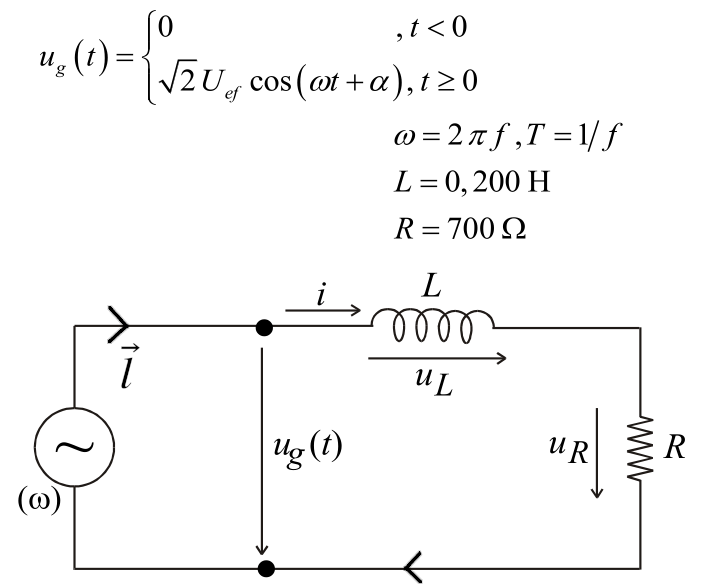
\includegraphics[width=0.7\linewidth]{rl.png}
			\caption{Circuito RL série em estudo, em que $f = \SI{5}{\kilo\hertz}$ e $U_{ef} = \SI{2}{\volt}$}
			\label{fig:circ_rl}
		\end{figure}
		\par
		Por aplicação da lei de indução no caminho $\vec{l}$ assinalado na \autoref{fig:circ_rl} e desprezando efeitos resistivos fora da resistência temos
		\begin{align*}
			&\ointclockwise_{\vec{l}} \vec{E} \vdot \dd{\vec{l}} = - \dv{\psi_{\vec{l}}}{t} \\ \eq
			&0 + u_R(t) - u_g(t) = - \dv{\psi_{\vec{l}}}{t} \\ \eq
			&u_g(t) = Ri(t) + N \dv{\phi}{t},
		\end{align*}
		onde $N$ é o número de espiras da bobina e $\phi$ o fluxo que atravessa cada uma das espiras. Considerando o circuito linear temos ainda
		\begin{align*}
			&N \dv{\phi}{t} = L \dv{i(t)}{t} \\ \implies
			&u_g(t) = Ri(t) + L \dv{i(t)}{t}. \numberthis \label{eq:trans_RL}
		\end{align*}
		\par
		Em $t = 0$ o gerador é ligado. Como $i(t)$ é uma variável de estado, pela continuidade da energia magnética na bobina, terá um regime transitório. A solução do regime transitório da corrente $i(t)$, dado por \eqref{eq:trans_RL}, é a soma do regime livre homogéneo (sem fontes) e do regime forçado estabelecido pelo gerador sinusoidal (quando $t \to \infty$), ou seja, $i(t) = i_l(t) + i_f(t)$.
		\par
		O regime forçado é então dado por
		\begin{align*}
			&\sqrt{2}U_{ef}\cos\left(\omega t + \alpha\right) = Ri_f(t) + L \dv{i_f(t)}{t}
		\end{align*}
		e em amplitude complexa
		\begin{align*}
			&\bar{U}_g = R\bar{I}_f + \jj \omega L\bar{I}_f \\ \eq
			&\dfrac{\bar{U}_g}{\bar{I}_f} = \bar{Z} = R + \jj \omega L = Z\e^{\jj\varphi},
		\end{align*}
		onde
		\begin{align*}
			&Z = \sqrt{R^2 + (\omega L)^2} \\
			&\varphi = \arctan\left(\dfrac{\omega L}{R}\right),
		\end{align*}
		o que nos permite finalmente resolver em ordem a $\bar{I}_f$ e $i_f(t)$
		\begin{align*}
			&\bar{I}_f = \dfrac{\bar{U}_g}{\bar{Z}} = \dfrac{\sqrt{2}U_{ef}}{Z} e^{\jj\left(\alpha - \varphi\right)} \\ \implies
			&i_f(t) = \Re{\bar{I}_f \e^{\jj \omega t}} = \Re{\dfrac{\sqrt{2}U_{ef}}{Z} \e^{\jj\left(\omega t + \alpha - \varphi\right)}} = \\ \eq
			&i_f(t) = \dfrac{\sqrt{2}U_{ef}}{Z} \cos\left(\omega t + \alpha - \varphi\right),
		\end{align*}
		em que $- \varphi = \SI{-1.46}{\radian} = \SI{-83.6}{\degree}$ é a desfasagem entre a tensão $u_g(t)$ e $i(t)$ em regime forçado.
		\par
		O regime livre é a solução da equação homogénea de \eqref{eq:trans_RL}
		\begin{align*}
			0 = R i(t) + L \dv{i(t)}{t}. \numberthis \label{eq:trans_RL_hom}.
		\end{align*}
		\par
		A equação diferencial em \eqref{eq:trans_RL_hom} tem uma solução do tipo exponencial e, portanto, substituindo $i(t) = \e^{st}$, a sua equação característica é
		\begin{align*}
			&0 = R\e^{st} + L\dv{\e^{st}}{t} \\ \eq
			&0 = R + Ls \\ \eq
			&s = - \dfrac{R}{L} = - \dfrac{1}{\tau},
		\end{align*}
		onde $\tau = \frac{L}{R} = \SI{0.286}{\milli\second}$ é a constante de tempo do circuito.
		\par
		A solução é então dada por
		\begin{align*}
			i_l(t) = I \e^{st} = I \e^{-\frac{t}{\tau}},
		\end{align*}
		onde a única constante de integração $I$ é determinada pela continuidade da corrente $i(t)$ na bobina
		\begin{align*}
			i(0^-) = i(0^+) = i_f(0^+) + i_l(0+).
		\end{align*}
		\par
		Dado que a corrente em $t < 0$ era nula e como $\alpha = \frac{\pi}{2}$
		\begin{align*}
			&0 =  \dfrac{\sqrt{2}U_{ef}}{Z} \cos\left(\omega 0 + \alpha - \varphi\right) + I \e^{-\frac{0}{\tau}} \\ \eq
			&I = - \dfrac{\sqrt{2}U_{ef}}{Z} \cos\left(- \frac{\pi}{2} - \varphi\right) = \SI{0.445}{\milli\ampere},
		\end{align*}
		sendo o regime transitório finalmente dado por
		\begin{gather*}
			i(t) = i_f(t) + i_l(t) = \\ =
			\dfrac{\sqrt{2}U_{ef}}{Z} \cos\left(\omega t + \alpha - \varphi\right) - \dfrac{\sqrt{2}U_{ef}}{Z} \cos\left(- \frac{\pi}{2} - \varphi\right) \e^{-\frac{t}{\tau}} \\ \eq
			i(t) = \dfrac{\sqrt{2}U_{ef}}{Z} \left[ \cos\left(\omega t + \alpha - \varphi\right) - \cos\left(\alpha - \varphi\right)e^{-\frac{t}{\tau}}\right] . \numberthis \label{eq:trans_RL_sol}
		\end{gather*}

		\begin{figure}[H]
			\centering
			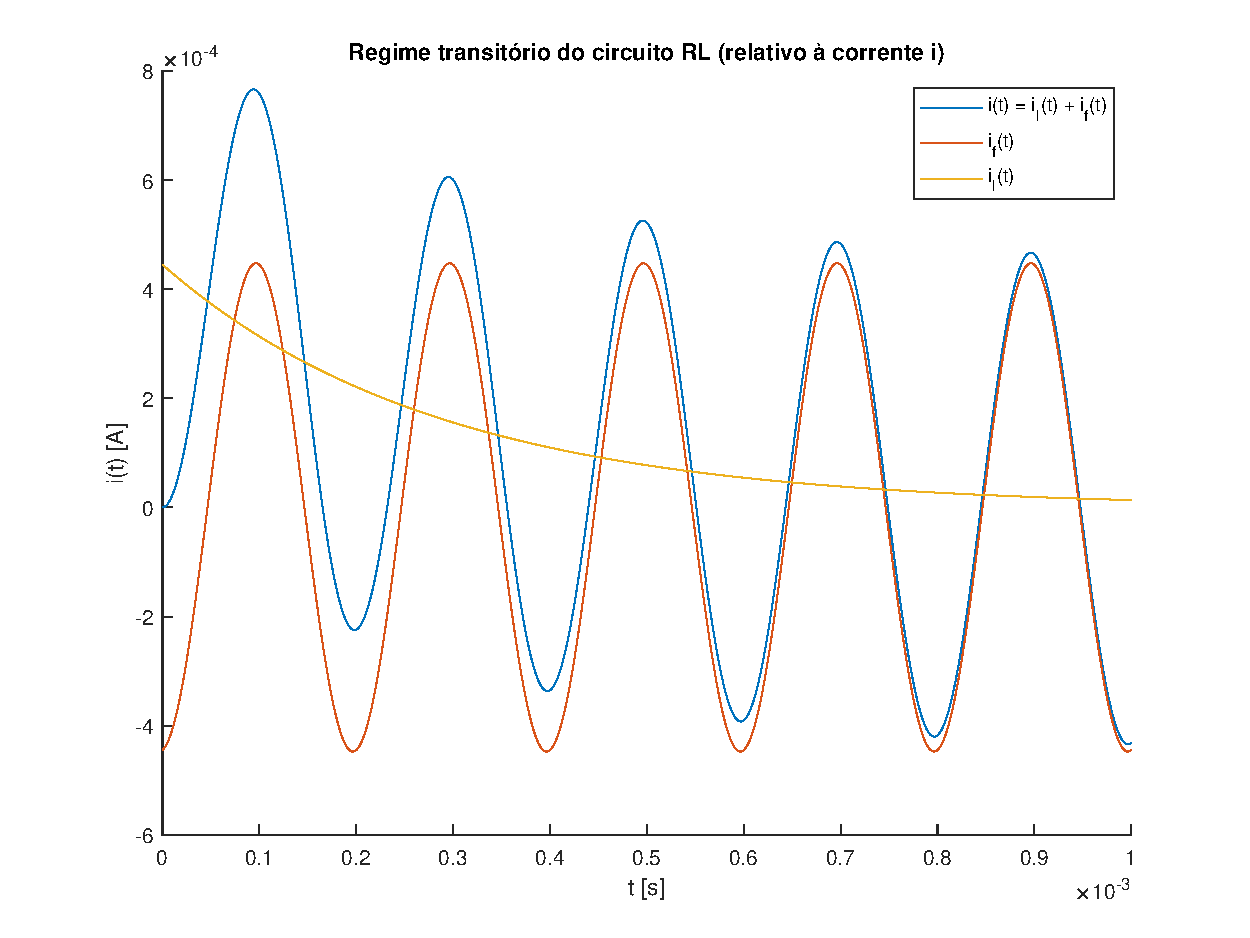
\includegraphics[width=1.0\linewidth]{rl.pdf}
			\caption{Gráfico do regime transitório da corrente $i(t)$ no circuito RL série}
			\label{fig:rl}
		\end{figure}

	% b)
	\subsubsection{}
	\par
	Supondo que os extermos do regime transitório de $i(t)$ em \eqref{eq:trans_RL_sol} se dão nos extremos da função cosseno, os instantes $t$ de extremo são dados por
	\begin{align*}
		&\cos\left(\omega t + \alpha - \varphi\right) = \pm 1 \\ \eq
		&\omega t + \alpha - \varphi = k\pi, k \in \mathbb{Z} \\ \eq
		&t = \dfrac{k\pi - \alpha + \varphi}{\omega}. \numberthis \label{eq:extr_insts}
	\end{align*}
	\par
	Substituindo \eqref{eq:extr_insts} em \eqref{eq:trans_RL_sol} obtemos, considerando $\alpha = -\dfrac{\pi}{2}$
	\begin{align*}
		i(t) = \dfrac{\sqrt{2}U_{ef}}{Z} \left[(-1)^k - \cos\left(-\dfrac{\pi}{2} - \varphi\right)\exp{-\dfrac{k\pi + \dfrac{\pi}{2} + \varphi}{\omega\tau}}\right].\numberthis \label{eq:extr}
	\end{align*}

	% c)
	\subsubsection{}
	\par
	Recorrendo ao \textit{matlab}, a partir de \eqref{eq:extr}, calcularam-se os primeiros cinco extremos da corrente em regime transitório $i(t)$ e registaram-se os valores na \autoref{tab:extremos}.
	\begin{table}[H]
		\centering
		\caption{Cinco primeiros extremos da corrente $i(t)$}
		\label{tab:extremos}
		\begin{tabular}{| r | r | S |}
			\hline
			\textbf{k} & \textbf{t} [\si{\milli\second}] & \textbf{i(t)} [\si{\milli\ampere}] \\
			\hline
			0 & 0.096 & 0.765 \\
			1 & 0.196 & -0.224 \\
			2 & 0.296 & 0.605 \\
			3 & 0.396 & -0.336 \\
			4 & 0.496 & 0.526 \\
			\hline
		\end{tabular}
	\end{table}
	\par
	Pelo método númerico de Newton, testa-se a validade da hipótese dos extremos de \eqref{eq:trans_RL_sol} se darem nos extremos da função cosseno apenas (desprezando o fator exponencial). Este método é iterativamente dado por
	\begin{align*}
		x_{n+1} = x_n - \dfrac{f(x_n)}{f'(x_n)}
	\end{align*}
	para uma função $f(x) = 0$ qualquer.
	\par
	Os extremos de $i(t)$ dão-se quando $i'(t) = 0$, logo será esta a função $f(x)$ a utlizar no método de Newton. Para tal ainda é necessário a derivada de $i'(t)$
	\begin{align*}
		&i'(t) = \dfrac{\sqrt{2}U_{ef}}{Z} \left[-\omega \sin\left(\omega t + \alpha - \varphi\right) + \dfrac{\cos\left(\alpha - \varphi\right)}{\tau}\e^{-\frac{t}{\tau}}\right] \\
		&i''(t) = \dfrac{\sqrt{2}U_{ef}}{Z} \left[-\omega^2 \cos\left(\omega t + \alpha - \varphi\right) + \dfrac{\cos\left(\alpha - \varphi\right)}{\tau^2}\e^{-\frac{t}{\tau}}\right].
	\end{align*}
	\par
	Foi calculado o primeiro extremo por recurso ao \textit{matlab}, impondo um erro $\epsilon = \num{e-6} \geq \abs{x_{n+1} - x_n}$ e uma aproximação inicial de $t = \SI{0.090}{\milli\second}$ (o valor aproximado obtido por \eqref{eq:extr_insts} foi $t = \SI{0.096}{\milli\second}$). O método de Newton convergiu para $t = \SI{0.09393}{\milli\second}$ em três iterações, o que significa que a aproximação apresenta um erro de apenas $\SI{2.07}{\micro\second}$ ou um erro relativo de $0.22\%$. Conclui-se assim que a aproximação é válida.

	% d)
	\subsubsection{}

	% e)
	\subsubsection{}

	% 2.2
	\subsection{Circuito RLC-série}
	\subsection{}
		\begin{figure}[H]
			\centering
			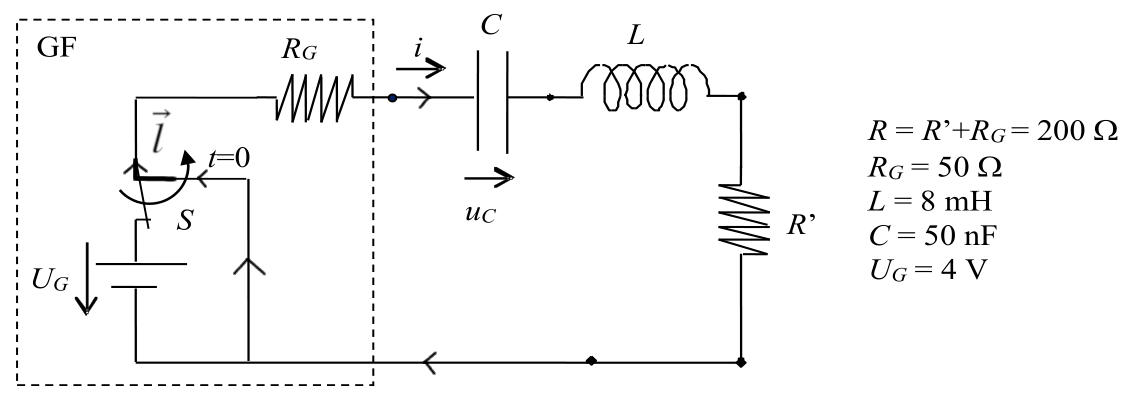
\includegraphics[width=0.7\linewidth]{rlc.png}
			\caption{Circuito RLC série em estudo, em que $f = \SI{5}{\kilo\hertz}$ e $U_{ef} = \SI{2}{\volt}$}
			\label{fig:circ_rlc}
		\end{figure}
	% a)
	\subsubsection{}

		\par
		Para $t \geq 0$, não existe a fonte de alimentação ($U_G = 0$) e portanto, ao aplicar a Lei da Indução (considerando o circuito linear), obtém-se

		\begin{align*}
			&\ointclockwise_{\vec{l}} \vec{E} \vdot \dd{\vec{l}} = - \dv{\psi_{\vec{l}}}{t} \\ \eq
			&u_R(t) + u_C(t) + 0 = - \dv{\psi_{\vec{l}}}{t} \\ \eq
			&Ri(t) + \frac{1}{C} \int i(t) dt + 0 = -L \dv{i(t)}{t} \\ \eq
			&L \dv{i(t)}{t} + Ri(t) + \frac{1}{C} \int i(t) dt = 0 \\
		\end{align*}

		Fazendo a derivada em ordem ao tempo, obtém-se a equação diferencial de segunda ordem dada por

		\begin{align*}
			&L \dv[2]{I(t)}{t} + R\dv{I(t)}{t} + \frac{1}{C}i(t) = 0 \\ \eq
			&\dv[2]{I(t)}{t} + 2\frac{R}{2L}\dv{i(t)}{t} + \frac{1}{LC}i(t) = 0 \\ \eq
			&\dv[2]{I(t)}{t} + 2\beta \dv{i(t)}{t} + \omega_{0}^{2} i(t) = 0, \numberthis \label{eq_dif_2ordem}
		\end{align*}

		sendo $\beta$ o coeficiente de amortecimento e $\omega_{0}$ a frequência angular das oscilações não amortecidas. Assim, o valor de $\omega_{0}$ é dado por

		\begin{align*}
			\omega_{0} = \frac{1}{\sqrt{LC}} = \SI{50e3}{\radian\per\second}.
		\end{align*}

	% b)
	\subsubsection{}

		\par
		Sendo necessária a continuidade da energia elétrica no condensador e da energia magnética na bobina, a tensão no condensador e a corrente na bobina têm de ser idênticos no instante imediatamente antes à comutação do interruptor $S$ e no instante imediatamente depois, ou seja
		\begin{align*}
			u_{C}(0^{+}) &= u_{C}(0^{-})\\
			  i_{L}(0^{+}) &= i_{L}(0^{-}).
		\end{align*}

		Tendo sido estabelecida a tensão estacionária do condensador, não existe corrente no circuito, portanto tem-se
		\begin{align*}
			i(0^{+}) = i(0^{-}) = \SI{0}{\ampere}. \numberthis \label{cond_inicial_corrente}
		\end{align*}

		Consequentemente, não havendo corrente no circuito, a tensão fornecida pela fonte estará aos terminais do condensador, obtendo assim
		\begin{align*}
			u_{C}(0^{+}) = u_{C}(0^{-}) = \SI{4}{\volt}. \numberthis \label{cond_inicial_tensão}
		\end{align*}

		Para $t > 0$, devido à comutação do interruptor $S$, o novo circuito deixa de estar alimentado, havendo apenas regime livre, não existindo regime forçado, ou seja $i_f(t) = 0$.

	% c)
	\subsubsection{}

		\par
		Existindo apenas regime livre, fazendo $i(t) = e^{st}$ em \ref{eq_dif_2ordem}, obtém-se a equação característica dada por
		\begin{align*}
			&s^{2} + 2\beta s + \omega_{0}^{2} = 0 .\numberthis \label{eq_caract_2ordem_sol}
		\end{align*}

		Aplicando a fórmula resolvente, obtém-se as raízes da equação \ref{eq_caract_2ordem_sol}, dadas por
		\begin{align*}
			&s =   -\beta \pm \sqrt{ \beta^{2} - \omega_{0}^{2}}, \numberthis \label{sol_eq_caract_2ordem}
		\end{align*}

		originando 3 soluções distintas.

		\begin{itemize}
			\item $\beta > \omega_{0} \implies \frac{R}{2L} > \frac{1}{\sqrt{LC}} \eq R > 2
			\sqrt{\frac{L}{C}}$, gerando um regime aperiódico

			\item $\beta = \omega_{0} \implies \frac{R}{2L} = \frac{1}{\sqrt{LC}} \eq R = 2
			\sqrt{\frac{L}{C}}$, gerando um regime aperiódico limite

			\item $\beta < \omega_{0} \implies \frac{R}{2L} < \frac{1}{\sqrt{LC}} \eq R < 2
			\sqrt{\frac{L}{C}}$, gerando um regime oscilatório amortecido
		\end{itemize}

	% d)
	\subsubsection{}

		\par
		Para $R = \SI{200}{\ohm} $, obtém-se $\beta = \frac{200}{2 \times \num{8e-3}} = \SI{12.5e3}{\neper\per\second}$. Como $\beta < \omega_{0}$, verifica-se que a solução é do tipo oscilatório amortecido. Sendo do tipo oscilatório amortecido, de \ref{sol_eq_dif_2ordem} retira-se
		\begin{align*}
			&s =   -\beta \pm \jj \omega,
		\end{align*}

		onde $\omega = \sqrt{\omega_{0}^{2} - \beta^{2}}$ é a frequência angular das oscilações amortecidas. Assim, o valor deste é dado por
		\begin{align*}
			\omega = \sqrt{\omega_{0}^{2} - \beta^{2}} \approx \SI{48.412e3}{\radian\per\second}.
		\end{align*}

		Uma vez que a solução da equação característica são 2 raízes complexas conjugadas, a solução da equação diferencial é dada por
		\begin{align*}
			&i(t) = \bar{I_1}\e^{st} + \bar{I_2}\e^{s^{*}t}
		\end{align*}

		Como i(t) é real, $\bar{I_{1}}$ e $\bar{I_{2}}$ são necessariamente complexos conjugados. Definindo $\bar{I} = 2\bar{I_1} = I\e^{j\alpha}$, tem-se
		\begin{align*}
			& i(t) = \Re{\bar{I}\e^{st}} \\ \eq
			& i(t) = \Re{I\e^{j\alpha}\e^{(-\beta + j\omega)t}} \\ \eq
			& i(t) = \Re{I\e^{-\beta t}\e^{j(\omega t + \alpha)}} \\ \eq
			& i(t) = I\e^{-\beta t} \cos{(\omega t + \alpha)}. \numberthis \label{sol_eq_dif_2ordem}
		\end{align*}

		Verifica-se que, de \ref{sol_eq_dif_2ordem}, a corrente i(t) terá amplitudes máximas (em módulo) quando o valor do coseno for máximo ou mínimo. Considerando a corrente i(t) apresentada na figura (INSERT REF), verifica-se que os valores absolutos dos máximos da função são dados por
		\begin{gather*}
			 A_1 = I\e^{-\beta \frac{T}{4}} \\
			 A_2 = I\e^{-\beta(\frac{T}{4} + \frac{T}{2})} \\
			 A_3 = I\e^{-\beta(\frac{T}{4} + T)}\\
			\vdots \\
			 A_n = I\e^{-\beta(\frac{T}{4} + (n-1)\frac{T}{2})} \\
			 \implies \frac{A_1}{A_n} = \frac{\cancel{I\e^{-\beta \frac{T}{4}}}}{\cancel{I\e^{-\beta\frac{T}{4}}} \e^{-\beta(n-1)\frac{T}{2}}} = \e^{\beta(n-1)\frac{T}{2}} \\ \eq
			 \left(\frac{A_1}{A_n}\right)^{\frac{1}{(n-1)}} = \e^{\beta\frac{T}{2}} = \e^\lambda,
		\end{gather*}

		sendo $\lambda$ o decremento logarítmico, dado por
		\begin{align*}
			 \lambda = \beta \frac{T}{2} = \SI{0.811}{\neper}.
		\end{align*}

		Tendo em conta as condições iniciais estabelecidas em \eqref{cond_inicial_corrente} e \eqref{cond_inicial_tensão}, é possível determinar a corrente i(t) e a tensão $u_{C}$. Para determinar a constante de integração de i(t), recorre-se ao regime forçado quando $t < 0$. Assim, da aplicação da Lei da Indução no caminho $l$ previamente escolhido, obtém-se 
		\begin{gather*}
			u_R(t) + u_C(t) + 0 = - \dv{\psi_{\vec{l}}}{t} \\ \eq
			u_C(t) = -Ri(t) - L\dv{i(t)}{t} \numberthis \label{eq_Uc_lei_ind} \\ \eq 
			u_C(t) = -R \left[ I\e^{-\beta t} \cos{(\omega t + \alpha)} \right] - L \left[ -\beta I\e^{-\beta t} \cos{(\omega t + \alpha)} - \omega I\e^{-\beta t} \sin{(\omega t + \alpha)}\right] \numberthis \label{eq_Uc_RLC}
		\end{gather*}
		
		De \eqref{cond_inicial_corrente}, retira-se 
		\begin{gather*}
			 i(0) = I\e^{-\beta \times 0} \cos{(\omega \times 0 + \alpha)} = 0 \\ \eq
			 I\cos{(\alpha)} = 0 \implies \alpha = \pm \frac{\pi}{2}
		\end{gather*}
		
		Considerando $\alpha =  \frac{\pi}{2}$, é possível determinar a expressão da tensão $u_{C}(t)$, tendo então 
		\begin{gather*}
			u_C(t) = -R \left[ I\e^{-\beta t} \cos{\left(\omega t + \frac{\pi}{2}\right)} \right] - L \left[ -\beta I\e^{-\beta t} \cos{\left(\omega t + \frac{\pi}{2}\right)} - \omega I\e^{-\beta t} \sin{\left(\omega t + \frac{\pi}{2}\right)}\right] \\ \eq
			u_C(t) = I\e^{-\beta t} \left[ \left( -R +\beta L\right) \cos{\left(\omega t + \frac{\pi}{2}\right)}  + \omega L\sin{\left(\omega t + \frac{\pi}{2}\right)} \right] \numberthis \label{Uc_RLC}
			\end{gather*}
			
		De \eqref{cond_inicial_tensão} e de \eqref{Uc_RLC}, retira-se 
		\begin{gather*}
			u_{C}(0) = I\e^{-\beta \times 0} \left[ \cancelto{0}{\left( -R +\beta L\right) \cos{\left(\omega \times 0 + \frac{\pi}{2}\right)}}  + \omega L \cancelto{1}{\sin{\left(\omega \times 0 + \frac{\pi}{2}\right)}} \right] = 4 \\ \eq
			 I\omega L = 4 \eq I = \frac{4}{\omega L} \implies I \approx \SI{10.328e-3}{\ampere}.
		\end{gather*}
		
		Por fim, obtém-se a expressão da tensão $u_{C}(t)$ e de $i(t)$, com as devidas aproximações, dadas por
		
		\begin{equation}
   			\begin{cases}
      			i(t) &\approx \num{10.328e-3}\e^{-\num{12.5e3}t} \cos{(\num{48.412e3} t + \frac{\pi}{2})} \\
    			\\u_C(t) &\approx \num{10.328e-3}\e^{-\num{12.5e3} t} \left[ -100 \cos{\left(\num{48.412e3} t + \frac{\pi}{2}\right)}  + \num{387.296}\sin{\left(\num{48.412e3}t + \frac{\pi}{2}\right)} \right] \\ 
			&\approx \num{1.0328e-3}\e^{-\num{12.5e3} t} \cos{\left(\num{48.412e3} t + \frac{\pi}{2}\right)}  + \num{4}\sin{\left(\num{48.412e3}t + \frac{\pi}{2}\right)}
  			\end{cases}       
		\end{equation}
		
	% e)
	\subsubsection{}
	
		\par
		De modo a que a solução do regime livre seja do tipo aperiódico limite, é necessário que $\beta = \omega_{0}$. Assim, utilizando a resolução da alínea c), tem-se 
		\begin{align*}
			 R_0 = R = 2\sqrt{\frac{L}{C}} = \SI{800}{\ohm}.
		\end{align*}
		
		Assim, equação característica \eqref{eq_caract_2ordem_sol} tem 2 raízes reais iguais, ou seja multiplicidade 2, e, portanto, a solução da equação diferencial é dada por
		\begin{align*}
			i ( t ) = ( A + B t ) \e ^ { s t }, \numberthis \label{eq_i_regime_ap_limite}
		\end{align*}

		onde, de \eqref{sol_eq_caract_2ordem}, tendo $\beta = \omega_{0}$, se obtém $s = - \beta$.
		
		De \eqref{cond_inicial_corrente}, retira-se 
		\begin{gather*}
			( A + B \times 0 ) \e ^ { - \beta \times 0 } = 0 \implies A = 0. \\ \eq
			i(t) = Bt\e^{-\beta t} \numberthis \label{eq_i_regime_ap_limite_2}
		\end{gather*}
		
		Substituindo \eqref{eq_i_regime_ap_limite_2} em \eqref{eq_Uc_lei_ind}, obtém-se
		\begin{align*}
			 u_C(t) &= -R\left(Bt\e^{-\beta t}\right) - L\left( B\e^{-\beta t} -\beta Bt\e^{-\beta t} \right) \\ \eq
			u_C(t)  &= B\e^{-\beta t} \left(  -Rt - L +\beta t  \right)
		\end{align*}
		
		De \eqref{cond_inicial_tensão}, retira-se 
		\begin{align*}
			 u_C(0)  &= B\e^{-\beta \times 0} \left(  -R\times 0 - L +\beta \times 0  \right) = 4 \\ \eq 
			 -BL &= 4 \eq B = \frac{-4}{L} = -500.
		\end{align*}
		
		Assim, tendo o valor de ambas as constantes de integração e fazendo a substituição em \eqref{eq_i_regime_ap_limite}, obtém-se finalmente a expressão da corrente $i(t)$, dada por 
		\begin{align*}
			i(t) = -500t\e^{-\num{50e3}t} \si{\ampere}. \numberthis \label{eq_i(t)_final}
		\end{align*}
		
		Fazendo a derivada em ordem ao tempo de \eqref{eq_i_regime_ap_limite_2} e igualando a 0, obtém-se o instante $t_{min}$ dado por
		\begin{gather*}
			\dv{i(t)}{dt} = B\left( \e^{-\beta t} - \beta t e^{-\beta t}\right) = 0 \\ \eq
			e^{-\beta t} = \beta t\e^{-\beta t} \\ \eq
			t = \frac{1}{\beta} = \SI{20}{\micro\second}.
		\end{gather*}
		
		Substituindo em \eqref{eq_i(t)_final}, obtém-se o valor de $i(t_{min})$
		\begin{gather*}
			i(t_{min}) = -500t_{min}\e^{-\num{50e3}t_{min}} = \SI{-3.679}{\milli\ampere}.
		\end{gather*}
		
	%Ver \autoref{fig:figure-example}

	%\printbibliography

\end{document}
